\section{Results}
\label{sec:results}

All results in \cref{sec:results:factors-structure,sec:results:baseline,sec:results:variants,sec:results:factors,sec:results:band}
are in-sample (\InSampleStart{} to 31~December~2018). \Cref{tab:main} summarises the main
variants. \Cref{app:variants} lists all \NVariants{} variants evaluated.

\begin{table}[ht]
\centering
\caption{In-sample performance of selected variants at 5~bps one-way cost. SR: annualised
Sharpe ratio. Net return: annualised, as a fraction of capital. Max DD: maximum drawdown of
cumulative net P\&L. Turnover: mean daily one-way turnover in units of capital. BE: break-even
one-way cost (\cref{eq:breakeven}).}
\label{tab:main}
\small
\setlength{\tabcolsep}{4pt}
\begin{tabular}{@{}lrrrrrr@{}}
\toprule
Variant & Gross SR & Net SR & Net return & Max DD & Turnover & BE (bps)\\
\midrule
AL baseline ($m=15$, daily hedge) & 1.33 & \ensuremath{-}1.18 & \ensuremath{-}4.0\% & \ensuremath{-}33.1\% & 0.67 & 2.6\\
Frozen hedge & 1.16 & \ensuremath{-}1.10 & \ensuremath{-}3.7\% & \ensuremath{-}31.6\% & 0.61 & 2.6\\
Volume-adjusted signal & 1.29 & \ensuremath{-}1.15 & \ensuremath{-}3.8\% & \ensuremath{-}30.4\% & 0.63 & 2.6\\
Wider entry ($\bar s_{\text{open}}=2.0$) & 0.83 & \ensuremath{-}1.14 & \ensuremath{-}2.1\% & \ensuremath{-}17.0\% & 0.28 & 2.1\\
$m=3$ & 1.29 & 0.09 & 0.4\% & \ensuremath{-}9.1\% & 0.41 & 5.4\\
$m=3$, band $0.0005$ & 1.24 & 0.17 & 0.7\% & \ensuremath{-}7.6\% & 0.36 & 5.8\\
$m=8$, band $0.002$ & 1.44 & 0.15 & 0.6\% & \ensuremath{-}7.5\% & 0.37 & 5.6\\
\bottomrule
\end{tabular}

\end{table}

\subsection{Factor structure}
\label{sec:results:factors-structure}

\Cref{fig:spectrum} shows the eigenvalue spectrum of the correlation matrix of \SpecN{} stocks
over the 252 days ending on the last in-sample day. The largest eigenvalue alone accounts for
\LamOneShare\% of total variance, and the 15 kept factors for \KeptShare\%. Only \NAboveEdge{}
eigenvalues exceed the Marchenko--Pastur edge of \MPEdge{}, the upper limit of the eigenvalue
distribution expected if returns were uncorrelated noise. So by this criterion, roughly half of
AL's 15 factors cannot be distinguished from noise at this date.

\begin{figure}[ht]
\centering
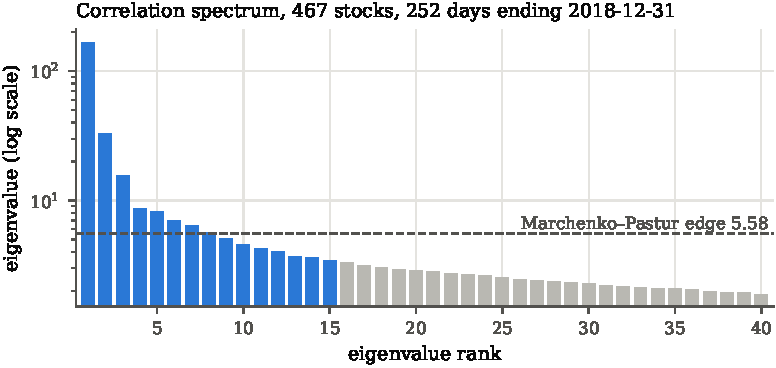
\includegraphics[width=\textwidth]{spectrum}
\caption{Leading 40 eigenvalues of the 252-day correlation matrix ending 31~December~2018 (log
scale). Blue bars are the 15 factors kept in the baseline. The dashed line is the
Marchenko--Pastur edge $(1+\sqrt{N/T})^2$ for $N=\SpecN$, $T=\SpecT$.}
\label{fig:spectrum}
\end{figure}

The leading eigenvectors have clear economic interpretations (\cref{fig:sectors}). The first
loads positively on every sector: it is the market. The second contrasts defensive,
interest-rate-sensitive sectors (utilities, real estate, consumer staples) with the rest of the
market. The third separates information technology from financials and energy, a growth-versus-value
pattern. The factors are therefore recognisable risk factors, even though PCA was not told
anything about sectors.

\begin{figure}[ht]
\centering
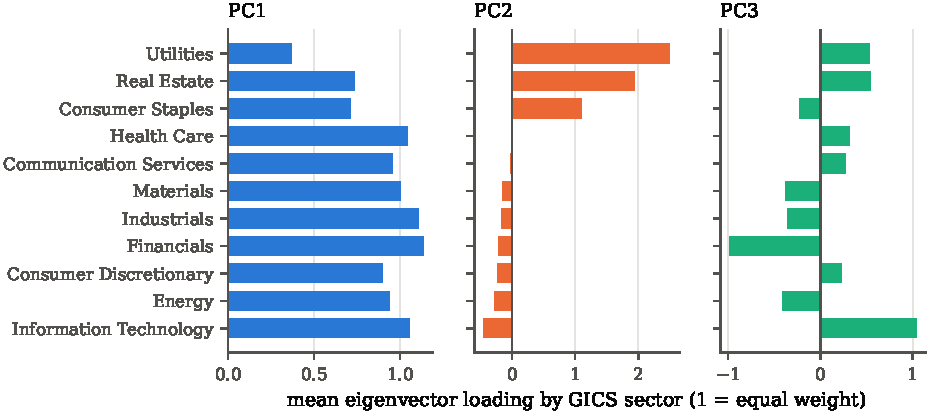
\includegraphics[width=\textwidth]{sector_loadings}
\caption{Mean eigenvector loading of the first three principal components by GICS sector, for the
same window as \cref{fig:spectrum}. Loadings are scaled by $\sqrt N$, so a value of 1 corresponds
to an equal-weighted portfolio.}
\label{fig:sectors}
\end{figure}

The share of variance explained by the 15 factors varies considerably over time
(\cref{fig:explained}). It averages \EVMean\% and ranges from \EVMin\% to \EVMax\%, peaking in
\EVMaxDate{}, when the trailing window covers the August 2011 sell-off and the European
sovereign debt crisis, a period of unusually high correlation across stocks. The amount of risk that is ``systematic'' is therefore itself time-varying, which argues
for choosing $m$ adaptively rather than fixing it.

\begin{figure}[ht]
\centering
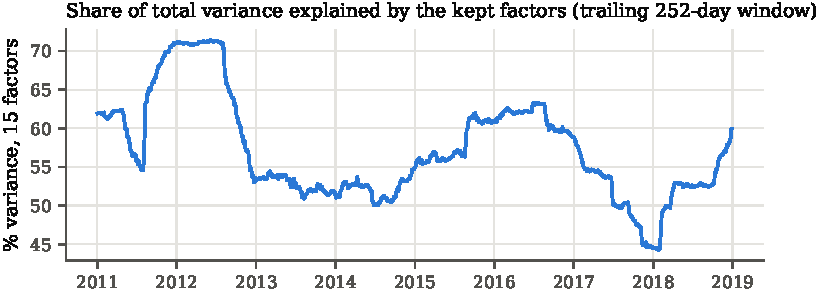
\includegraphics[width=\textwidth]{explained_variance}
\caption{Share of total variance explained by the 15 leading eigenvalues, using a trailing
252-day window.}
\label{fig:explained}
\end{figure}

\subsection{Baseline replication}
\label{sec:results:baseline}

\Cref{fig:sscore} illustrates the trading rule for one stock. The s-score of JPMorgan Chase
fluctuates within roughly $\pm 2$, and positions are opened when it crosses $\pm 1.25$ and closed
as it reverts. Across the in-sample period an average of \BaseOpenMean{} positions are open, and a
position is held for about \BaseHolding{} trading days.

\begin{figure}[ht]
\centering
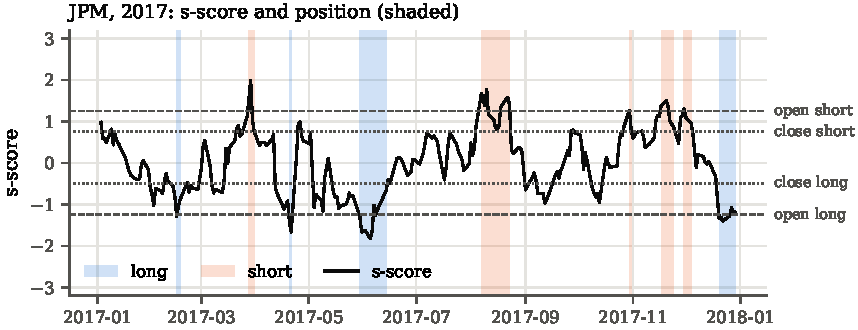
\includegraphics[width=\textwidth]{sscore_example}
\caption{s-score of JPMorgan Chase (JPM) in 2017 under the baseline specification, with entry
(dashed) and exit (dotted) thresholds. Shaded regions mark open long (blue) and short (orange)
positions.}
\label{fig:sscore}
\end{figure}

The baseline earns a gross annualised return of \BaseGrossRet\% with a volatility of
\BaseVol\%, i.e.\ a gross Sharpe ratio of \BaseGrossSR{} (\cref{fig:cumpnl}). The residual
mean-reversion signal is therefore still present in the S\&P~500 after 2010. After 5~bps
one-way costs, however, the annualised return is \BaseNetRet\% and the net Sharpe ratio
\BaseNetSR{}. The strategy trades \BaseTurnover{} times its capital per day, so it pays roughly
$0.67 \times 252 \times 5\,\text{bps} \approx 8.4\%$ a year in costs, about twice its gross
return. Equivalently, its gross edge is only \BaseBreakeven{}~bps per unit traded, half of the
assumed cost.

\begin{figure}[ht]
\centering
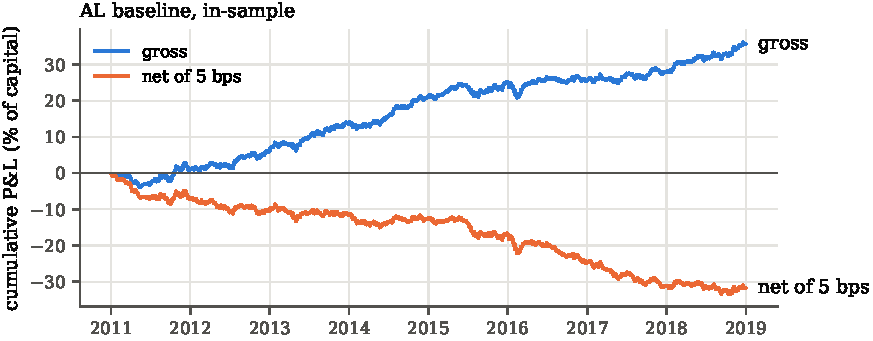
\includegraphics[width=\textwidth]{cum_pnl_baseline}
\caption{Cumulative in-sample P\&L of the baseline, gross and net of 5~bps one-way costs, as a
percentage of (fixed) capital.}
\label{fig:cumpnl}
\end{figure}

\paragraph{Where the turnover comes from.}
Of the \BaseTurnover{} daily turnover, \BaseStockLegTurnover{} is the stock leg, i.e.\ opening and
closing the positions themselves. The remaining \BaseHedgeTurnover{} is hedge trading. Hedging
therefore doubles the strategy's trading costs. As the next subsection shows, most of the hedge
turnover is \emph{not} the daily re-hedging of existing positions but the hedge baskets traded
when positions open and close.

\subsection{Hedge mode, volume adjustment and thresholds}
\label{sec:results:variants}

\paragraph{Frozen hedges} reduce turnover only from 0.67 to 0.61, and they lower the gross Sharpe
ratio from 1.33 to 1.16 because the hedges go stale. Daily re-hedging is therefore cheap: about
0.06 of turnover per day. The large hedge cost comes from building and unwinding the hedge
baskets, which frozen hedging does not change.

\paragraph{The volume-adjusted signal} leaves the break-even cost unchanged at 2.6~bps and
slightly lowers the gross Sharpe ratio (1.29). Combined with frozen hedges it performs worse
still (gross Sharpe 1.01). This contrasts with AL, who found that trading time improved
performance in 2003--2007.

\paragraph{Wider entry thresholds} cut turnover substantially, from 0.67 at
$\bar s_{\text{open}} = 1.25$ to 0.28 at $2.0$, but lower gross returns in proportion or more:
the break-even cost falls from 2.6 to 2.1~bps. Larger deviations are thus \emph{not} more
profitable per unit traded. Exiting later (at $s=0$ or beyond) does not help either. Changing the
residual window to 90 days or the $\kappa_{\min}$ filter also leaves the break-even cost at or
below the baseline (\cref{app:variants}).

\subsection{Number of factors}
\label{sec:results:factors}

The number of hedged factors is the most important design choice (\cref{fig:tradeoff}). The
gross Sharpe ratio rises from 0.74 with a single (market) factor to a maximum of 1.55 at
$m=8$, then falls to 1.33 at $m=15$ and 1.16 at $m=30$. Turnover rises steadily with $m$, from
0.36 to 1.09, because every additional factor adds a basket trade across the whole universe
whenever a position is opened or closed. The break-even cost is about 5~bps for $m \le 3$ and
declines for larger $m$, to 2.6~bps at AL's $m=15$ and 1.4~bps at $m=30$.

Two observations stand out. First, the gross Sharpe ratio peaks at $m=8$, the same number of
eigenvalues that exceed the Marchenko--Pastur edge in \cref{fig:spectrum}. Factors beyond the
noise edge seem to add estimation noise to the residuals rather than remove systematic risk.
Second, a few factors suffice to remove most of the systematic risk at a fraction of the hedging
cost.

\begin{figure}[ht]
\centering
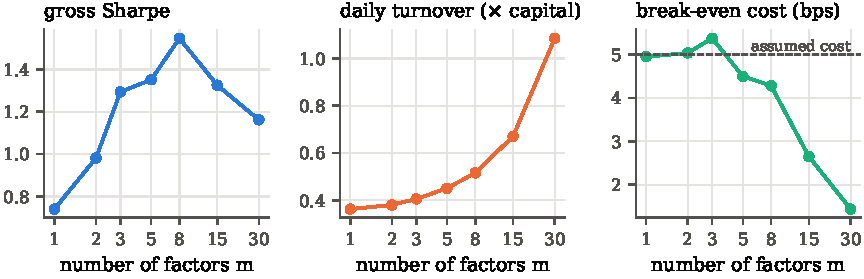
\includegraphics[width=\textwidth]{factor_tradeoff}
\caption{Gross Sharpe ratio, mean daily turnover and break-even cost as a function of the number
of hedged factors $m$ (log scale), in-sample. All other parameters at baseline values. The
dashed line marks the assumed cost of 5~bps.}
\label{fig:tradeoff}
\end{figure}

\subsection{No-trade band}
\label{sec:results:band}

The no-trade band reduces turnover for every number of factors at a small cost in gross Sharpe
ratio (\cref{tab:main} and \cref{app:variants}). With $m=15$, a band of $\delta = 0.002$ cuts
turnover from 0.67 to 0.49 and raises the break-even cost from 2.6 to 3.5~bps, which is still not
enough. Combined with fewer factors, the best in-sample variants reach break-even costs of
5.6--5.8~bps and net Sharpe ratios of about 0.15. Examples are $m=8$ with $\delta=0.002$ (gross
Sharpe 1.44) and $m=3$ with $\delta = 0.0005$ (gross Sharpe 1.24). These are modest numbers. After
correcting for the \NVariants{} variants tried, they are unlikely to be statistically
distinguishable from zero.

\subsection{Held-out test}
\label{sec:oos}

\todo{Pre-register the final variants (proposed: AL baseline; $m=8$ with $\delta=0.002$; $m=3$
with $\delta=0.0005$; plus phase-3 extensions), then run \code{experiments.py --reveal-test}
once and report the test-period performance, deflated Sharpe ratio and bootstrap confidence
intervals.}
